\documentclass{article}
\usepackage[paperwidth=360pt,paperheight=190pt,margin=0pt,noheadfoot]{geometry}
\usepackage{tikz}
\usetikzlibrary{calc}

\definecolor{ink}{RGB}{28,41,56}
\definecolor{axis}{RGB}{100,116,139}
\definecolor{grid}{RGB}{203,213,225}
\definecolor{curve}{RGB}{30,64,175}
\definecolor{teal}{RGB}{13,148,136}
\definecolor{tealfill}{RGB}{176,227,219}
% Integral diagrams use exactly one semantic palette: blue for the
% lower-only part, yellow for the upper-only (or still unresolved) part, and
% green for their common part.  The common part is explicit rather than an
% alpha blend, so the three meanings stay distinct after GIF quantization.
\definecolor{blue}{RGB}{0,114,178}
\definecolor{bluefill}{RGB}{86,180,233}
\definecolor{yellow}{RGB}{230,159,0}
\definecolor{yellowfill}{RGB}{255,218,102}
\definecolor{green}{RGB}{0,128,84}
\definecolor{greenfill}{RGB}{89,190,142}
\definecolor{orange}{RGB}{234,88,12}
\definecolor{orangefill}{RGB}{254,215,170}
\definecolor{purple}{RGB}{126,34,206}
\definecolor{yellowedge}{RGB}{202,138,4}
\definecolor{projection}{RGB}{148,163,184}
\colorlet{under}{blue}
\colorlet{underfill}{bluefill}
\colorlet{over}{yellow}
\colorlet{overfill}{yellowfill}
\colorlet{shared}{green}
\colorlet{sharedfill}{greenfill}
\colorlet{gap}{yellow}
\colorlet{gapfill}{yellowfill}

\pagestyle{empty}
\setlength\parindent{0pt}
\setlength\topskip{0pt}
\begin{document}
\noindent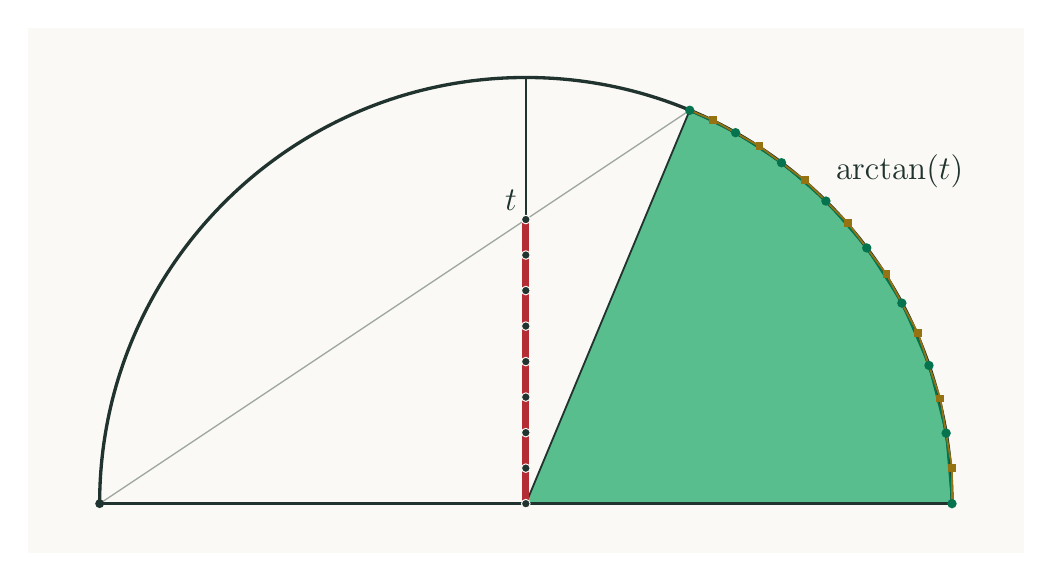
\begin{tikzpicture}[baseline=(current bounding box.north),x=1pt,y=1pt,line cap=round,line join=round]
\useasboundingbox (0,0) rectangle (360,190);
\definecolor{paper}{HTML}{FAF9F5}
\definecolor{semicircle}{HTML}{20332E}
\colorlet{lowerbound}{shared!85!semicircle}
\colorlet{upperbound}{yellow!59!semicircle}
\fill[paper] (0,0) rectangle (360,190);
\colorlet{lowerarea}{sharedfill}
\colorlet{upperarea}{overfill}
\colorlet{addition}{lowerbound!76!lowerarea}
\colorlet{cutoff}{yellow!85!upperarea}
\tikzset{chord/.style={lowerbound,line width=.65pt},tangent/.style={upperbound,line width=.65pt},chord trace/.style={chord,line width=1.25pt,dash pattern=on 5.5pt off 2.3pt},tangent trace/.style={tangent,line width=1.25pt,dash pattern=on 3.7pt off 2.2pt}}
\fill[upperarea] (180,18) -- (334,18) -- (334,30.8333) -- (329.7808,55.9726) -- (321.68,79.6) -- (310.3077,100.9231) -- (296.439,119.4146) -- (280.8966,134.8276) -- (264.4516,147.1613) -- (247.76,156.6) -- (239.2308,160.1538) -- cycle;
\fill[lowerarea] (180,18) -- (334,18) -- (331.8759,43.4897) -- (325.6757,67.9459) -- (315.8824,90.4706) -- (303.2,110.4) -- (288.4379,127.3491) -- (272.4,141.2) -- (255.8031,152.0518) -- (239.2308,160.1538) -- cycle;
\draw[semicircle,line width=.85pt] (26,18) -- (334,18);
\draw[semicircle,line width=1.2pt] (334,18) arc[start angle=0,end angle=180,radius=154pt];
\draw[semicircle,line width=.65pt] (180,18) -- (239.2308,160.1538);
\draw[semicircle!42!paper,line width=.5pt] (26,18) -- (239.2308,160.1538);
\draw[chord] (334,18) -- (331.8759,43.4897) -- (325.6757,67.9459) -- (315.8824,90.4706) -- (303.2,110.4) -- (288.4379,127.3491) -- (272.4,141.2) -- (255.8031,152.0518) -- (239.2308,160.1538);
\draw[tangent] (334,18) -- (334,30.8333) -- (329.7808,55.9726) -- (321.68,79.6) -- (310.3077,100.9231) -- (296.439,119.4146) -- (280.8966,134.8276) -- (264.4516,147.1613) -- (247.76,156.6) -- (239.2308,160.1538);
\fill[semicircle] (26,18) circle[radius=1.6pt];
\fill[lowerbound] (334,18) circle[radius=1.7pt];
\fill[lowerbound] (331.8759,43.4897) circle[radius=1.7pt];
\fill[lowerbound] (325.6757,67.9459) circle[radius=1.7pt];
\fill[lowerbound] (315.8824,90.4706) circle[radius=1.7pt];
\fill[lowerbound] (303.2,110.4) circle[radius=1.7pt];
\fill[lowerbound] (288.4379,127.3491) circle[radius=1.7pt];
\fill[lowerbound] (272.4,141.2) circle[radius=1.7pt];
\fill[lowerbound] (255.8031,152.0518) circle[radius=1.7pt];
\fill[lowerbound] (239.2308,160.1538) circle[radius=1.7pt];
\fill[upperbound] (332.6,29.4333) rectangle (335.4,32.2333);
\fill[upperbound] (328.3808,54.5726) rectangle (331.1808,57.3726);
\fill[upperbound] (320.28,78.2) rectangle (323.08,81);
\fill[upperbound] (308.9077,99.5231) rectangle (311.7077,102.3231);
\fill[upperbound] (295.039,118.0146) rectangle (297.839,120.8146);
\fill[upperbound] (279.4966,133.4276) rectangle (282.2966,136.2276);
\fill[upperbound] (263.0516,145.7613) rectangle (265.8516,148.5613);
\fill[upperbound] (246.36,155.2) rectangle (249.16,158);
\definecolor{inputsegment}{HTML}{B52D34}
\draw[semicircle,line width=.65pt] (180,18) -- (180,172);
\draw[inputsegment,line width=2.4pt] (180,18) -- (180,120.6667);
\filldraw[fill=semicircle,draw=paper,line width=.35pt] (180,18) circle[radius=1.55pt];
\filldraw[fill=semicircle,draw=paper,line width=.35pt] (180,30.8333) circle[radius=1.55pt];
\filldraw[fill=semicircle,draw=paper,line width=.35pt] (180,43.6667) circle[radius=1.55pt];
\filldraw[fill=semicircle,draw=paper,line width=.35pt] (180,56.5) circle[radius=1.55pt];
\filldraw[fill=semicircle,draw=paper,line width=.35pt] (180,69.3333) circle[radius=1.55pt];
\filldraw[fill=semicircle,draw=paper,line width=.35pt] (180,82.1667) circle[radius=1.55pt];
\filldraw[fill=semicircle,draw=paper,line width=.35pt] (180,95) circle[radius=1.55pt];
\filldraw[fill=semicircle,draw=paper,line width=.35pt] (180,107.8333) circle[radius=1.55pt];
\filldraw[fill=semicircle,draw=paper,line width=.35pt] (180,120.6667) circle[radius=1.55pt];
\node[anchor=south east,inner sep=1pt,text=semicircle,font=\large] at (178,122.6667) {\(t\)};
\node[anchor=west,inner sep=1pt,text=semicircle,font=\large] at (290.88,138.12) {\(\arctan(t)\)};
\end{tikzpicture}
\end{document}
